\chapter{Implementácia FPGA MITM obvodu}
\label{kap:implementacia}

V tejto kapitole navrhneme a implementujeme hardvérový MITM obvodu pomocou FPGA. Hlavným cieľom bude možnosť podpory pre viacero zbernicových protokolov a snaha o abstrakciu detailov fyzického protokolu zbernice pred samotnou MITM logikou obvodu. Ako sme v časti \ref{sek:masterSlave} spomenuli, niektoré vlastnosti principiálne nemožno abstrahovať. Napriek tomu ukážeme, že viacero vlastností možno pred vyššou vrstvou zakryť. Tento prístup zároveň umožní pomerne jednoduché rozšírenie o podporu ďalších zbernicových protokolov. V práci sa zameriame na konkrétne dva -- UART a SPI. Dôvodom výberu týchto dvoch zberníc je fakt, že princíp ich fungovania je značne odlišný ako sme detailnejšie uviedli v kapitole \ref{kap:zbernice}.

\section{Technické aspekty implementácie}
V tejto časti opíšeme po technickej stránke spôsob, ktorým sme sa rozhodli implementovať hardvérový MITM obvod. Obvod implementujeme pomocou FPGA technológie, ktorá umožňuje obvod flexibilne nakonfigurovať a upravovať podľa potreby. Výhodou oproti štandardnému softvérovému prístupu s využitím procesora pre všeobecné použitie (angl. general purpose) procesora je možnosť kontroly nad spracovaním informácie na úrovni logických hradiel. To umožňuje jednoduchšiu a najmä rýchlejšiu manipuláciu s fyzickou vrstvou signálov na zberniciach a ich spracovanie.

\subsection{Hardvér}
Čo sa týka hardvéru, v práci sme sa rozhodli pracovať s dvoma FPGA vývojovými doskami od spoločnosti Lattice Semiconductor, konkrétne ide o dosky iCEstick Evaluation Kit, ďalej len icestick a iCE40-HX8K Breakout Board, ďalej len doska HX8K. Na obrázku \ref{obr:iceHw} možno vidieť pohľad z vrchu na obidve dosky. Obidve dosky obsahujú čipy zo sady iCE40-HX. Vývojová doska icestick obsahuje lacnejší FPGA čip iCE40-HX1K, ktorý obsahuje pomerne málo logických buniek pre skladanie FPGA obvodu. Pre komplikovanejšie obvody, ktorých konfigurácia sa na tento FPGA čip nemusí zmestiť preto použijeme dosku HX8K, ktorá obsahuje čip iCE40-HX8K. Ten má približne osemkrát viac logických buniek, čo pre naše účely postačuje. Dôvodom výberu týchto vývojových dosiek je priamočiara podpora open source softvérových nástrojov pre syntézu FPGA kódu. Ďalej dosky obsahujú prevodník z USB na UART, ktorý umožňuje jednoduché nahranie výslednej konfigurácie obvodu na FPGA čip.

\begin{figure}
    \centering
    \subfloat[Icestick Evaluation Kit]{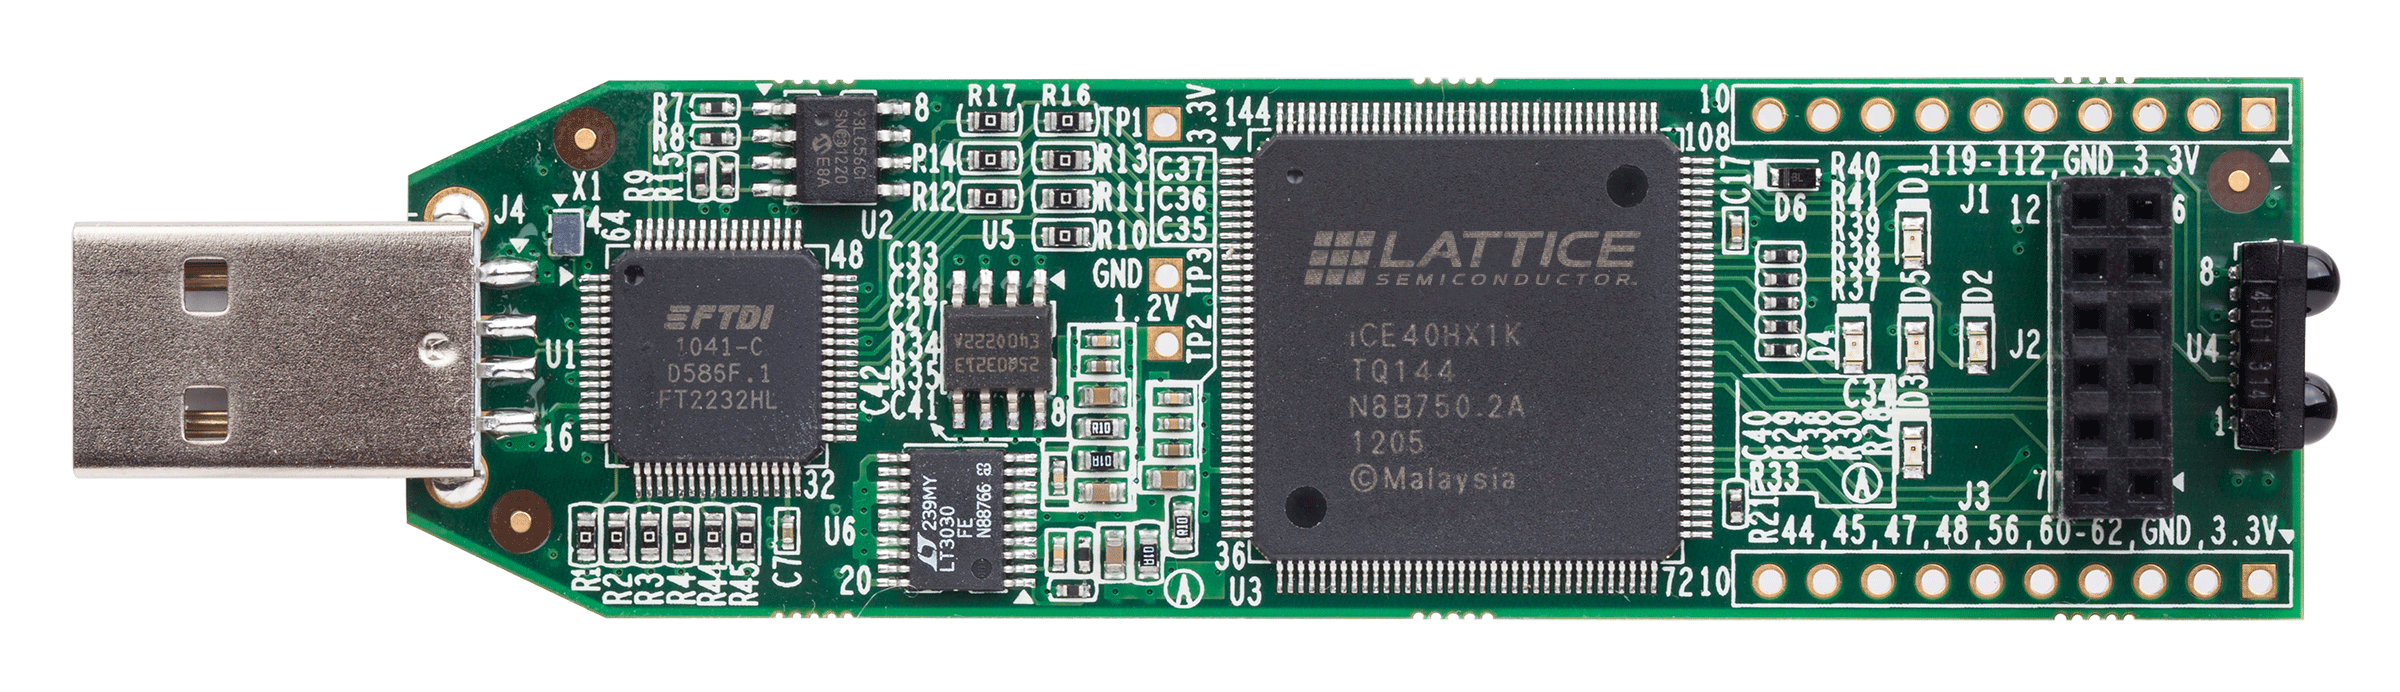
\includegraphics[width=0.6\textwidth]{images/misc/icestickHw.png}}
    \hfill
    \subfloat[iCE40-HX8K Breakout Board]{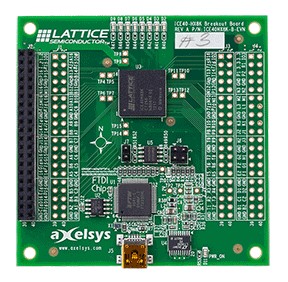
\includegraphics[width=0.4\textwidth]{images/misc/hx8kBoardHw.png}}
    \caption[Vývojové dosky FPGA iCE40]{Vývojové dosky FPGA iCE40. Zdroj: https://www.latticesemi.com}
    \label{obr:iceHw}
\end{figure}

\subsection{Programovací jazyk Verilog}
Existuje viacero jazykov pre popisovanie hardvéru, najrozšírenejšími sú VHDL a Verilog. MITM obvod sme sa rozhodli implementovať v jazyku Verilog. Dôvodom bola podpora jazyka open source nástrojmi, ktoré popíšeme v ďalšej časti. V nasledujúcich častiach podrobnejšie popíšeme spôsob implementácie nášho MITM obvodu. V týchto častiach predpokladáme, že čitateľ pozná syntax a základné princípy písania kódu v jazyku Verilog. Zdrojový kód celej implementácie sa nachádza v elektronickej prílohe priloženej k práci.

\subsection{Softvérové nástroje}\label{subsek:software}
Pre účely syntézy, testovania a simulácie kódu, sme využili viacero softvérových nástrojov. Všetky použité nástroje sú open source a sú zadarmo dostupné. V tejto časti jednotlivé nástroje stručne opíšeme:

\textbf{Yosys} (Yosys Open SYnthesis Suite) \cite{yosys} je hlavný nástroj, ktorý sme použili pre syntézu Verilog kódu. Jeho výstupom je tzv. netlist, ktorý reprezentuje výslednú FPGA konfiguráciu, presnejšie logické prepojenie jednotlivých komponentov na FPGA (logické bunky, pamäťové členy, vstupno-výstupné porty a pod.).

\textbf{NextPNR} (Next Place and Route) \cite{nextpnr} je ďalším nástrojom v reťazi, ktorého vstupom je netlist vygenerovaný predchádzajúcim nástrojom yosys. Tento nástroj má za úlohu naplánovať fyzické rozmiestnenie jednotlivých hardvérových komponentov a ich prepojenie pomocou vodičov. Pri tomto kroku je špeciálne dôležité naplánovať obvod tak, aby boli pri propagácii signálu medzi fyzickými časťami obvodu dodržané časové obmedzenia (angl. timing constraints). Výstup sa zvykne nazývať plánovaný (routed) netlist.

\textbf{Project IceStorm} \cite{icestorm} je sada nástrojov, pre prácu s FPGA obvodmi z rodiny iCE40, ktorý bol vyvinutý pomocou reverzného inžinierstva. V práci sme použili nasledovné nástroje z projektu IceStorm:\\
\textbf{icepack} -- posledný nástroj v \uv{kompilačnej} reťazi. Vstupom je plánovaný netlist vygenerovaný pomocou nextPNR. Tento vstup zakóduje do tzv. bitstreamu, čo je binárny formát, ktorý možno priamo nahrať na samotnú FPGA dosku.\\
\textbf{iceprog} -- nástroj, ktorý umožňuje nahrať výsledný bitstream na FPGA dosku.\\
\textbf{icetime} -- pomocný nástroj, ktorý overí dodržanie časových obmedzení. Vstupom je plánovaný netlist a výstupom je textová správa popisujúca výsledok overenia.\\
\textbf{icepll} -- pomocný nástroj, ktorý na základe vstupnej a požadovanej výstupnej frekvencie vypočíta potrebné parametre pre nastavenie PLL obvodu pre generovanie hodinového signálu. Výsledné parametre možno potom použiť priamo vo Verilog kóde pri inštanciácii PLL modulu.

\textbf{ICARUS Verilog} \cite{iverilog} je ďalším nástrojom, ktorý sme pri implementácii použili. Tento nástroj je podobne ako yosys syntetizátor Verilog kódu, jeho účelom nie je však generovanie fyzicky použiteľnej FPGA konfigurácie, ale simulácia FPGA obvodu. Výstupom je VVP (Verilog VPI Processor) kód, ktorý možno simulovať napríklad pomocou nástroja \textbf{vvp} (súčasťou projektu ICARUS Verilog). Výsledkom simulácie je súbor simulačných dát, napríklad vo VCD formáte.

\textbf{GTKWave} \cite{gtkwave} je nástroj, ktorý dokáže vizuálne reprezentovať priebeh signálov zo simulačných dát. Tento nástroj sme spolu s nástrojom ICARUS Verilog použili na testovanie a odhalenie logických chýb pri implementácii FPGA obvodu.

V nasledujúcich častiach detailnejšie opíšeme našu implementáciu jednotlivých častí FPGA obvodu.

\section{Hlavný modul obvodu}\label{sek:topLevelModule}
Celý obvod sa na najvyššej úrovni bude skladať z hlavného modulu (Top Level Module), ktorý zastrešuje celý obvod a obsahuje vstupy a výstupy, ktoré budú pripojené k fyzickým I/O portom. Všetky externé vstupy je potrebné synchronizovať. Synchronizácia zabezpečí, že všetky hrany (zmeny signálu z 0 na 1, resp. naopak) výsledného signálu budu synchrónne s globálnymi systémovými hodinami. Spôsob implementácie synchronizačného obvodu bližšie popíšeme v časti \ref{subsek:synchronizer}.

\subsection{Systémové hodiny}
Systémový hodinový signál, ďalej len systémové hodiny, je generovaný pomocou PLL obvodu. Využijeme PLL obvod, ktorý nám poskytuje knižnica pre prácu s iCE40 FPGA čipmi, podporovaná aj nami zvoleným yosys syntetizátorom. Ako referenčný vstup pre PLL obvod pripojíme 12\,MHz oscilátor, ktorý sa nachádza na obidvoch doskách icestick, resp. HX8K. Tento vstup, narozdiel od ostatných, nie je potrebné synchronizovať. Výstupnú frekvenciu PLL obvodu ponecháme ako voliteľný parameter, pričom podporované frekvencie sú z rozsahu 16 -- 275\,MHz.

Pre tento účel použijeme nástroj icepll spomenutý v časti \ref{subsek:software}, ktorý zo vstupnej a požadovanej výstupnej frekvencie dokáže vygenerovať priamo Verilog kód, ktorý inštancuje knižničný modul s potrebnými parametrami.
Tento proces využijeme pri automatizovanej syntéze kódu pomocou nástroja GNU make. Nie všetky hodnoty z rozsahu je možné dosiahnuť, v prípade, že požadovaná výstupná frekvencia nie je možná, nástroj vygeneruje kód, ktorý nakonfiguruje najbližšiu možnú frekvenciu k požadovanej.

\subsection{Ostatné časti obvodu}
Okrem generovania systémových hodín a synchronizácie vstupu bude hlavný modul pozostávať z troch dôležitých pod-modulov, ktorých implementáciu bližšie popíšeme v príslušných častiach. Prvým pod-modulom je rozhranie, ktoré zakrýva detaily zbernice (Bus Interface) a sú k nemu pripojené vstupy a výstupy zbernicových liniek oboch strán. I/O handler je modul pre spracovanie ostatných vstupov a výstupov netýkajúcich sa priamo zbernice, napr. tlačidlá pre globálny reset signál, žiadosť o zmenu režimu MITM logiky, LED indikujúca prebiehajúcu komunikáciu a pod. Posledným a najdôležitejším modulom je MITM logika, ktorú treba naprogramovať podľa konkrétneho útoku s využitím zbernicového rozhrania. Pri návrhu obvodu pre MITM logiku možno využiť vybrané vstupy z modulu I/O handler, pre dynamické nastavenie logiky. Schéma hlavného modulu je na obrázku \ref{obr:topLevelModule}.

\begin{figure}
    \centerline{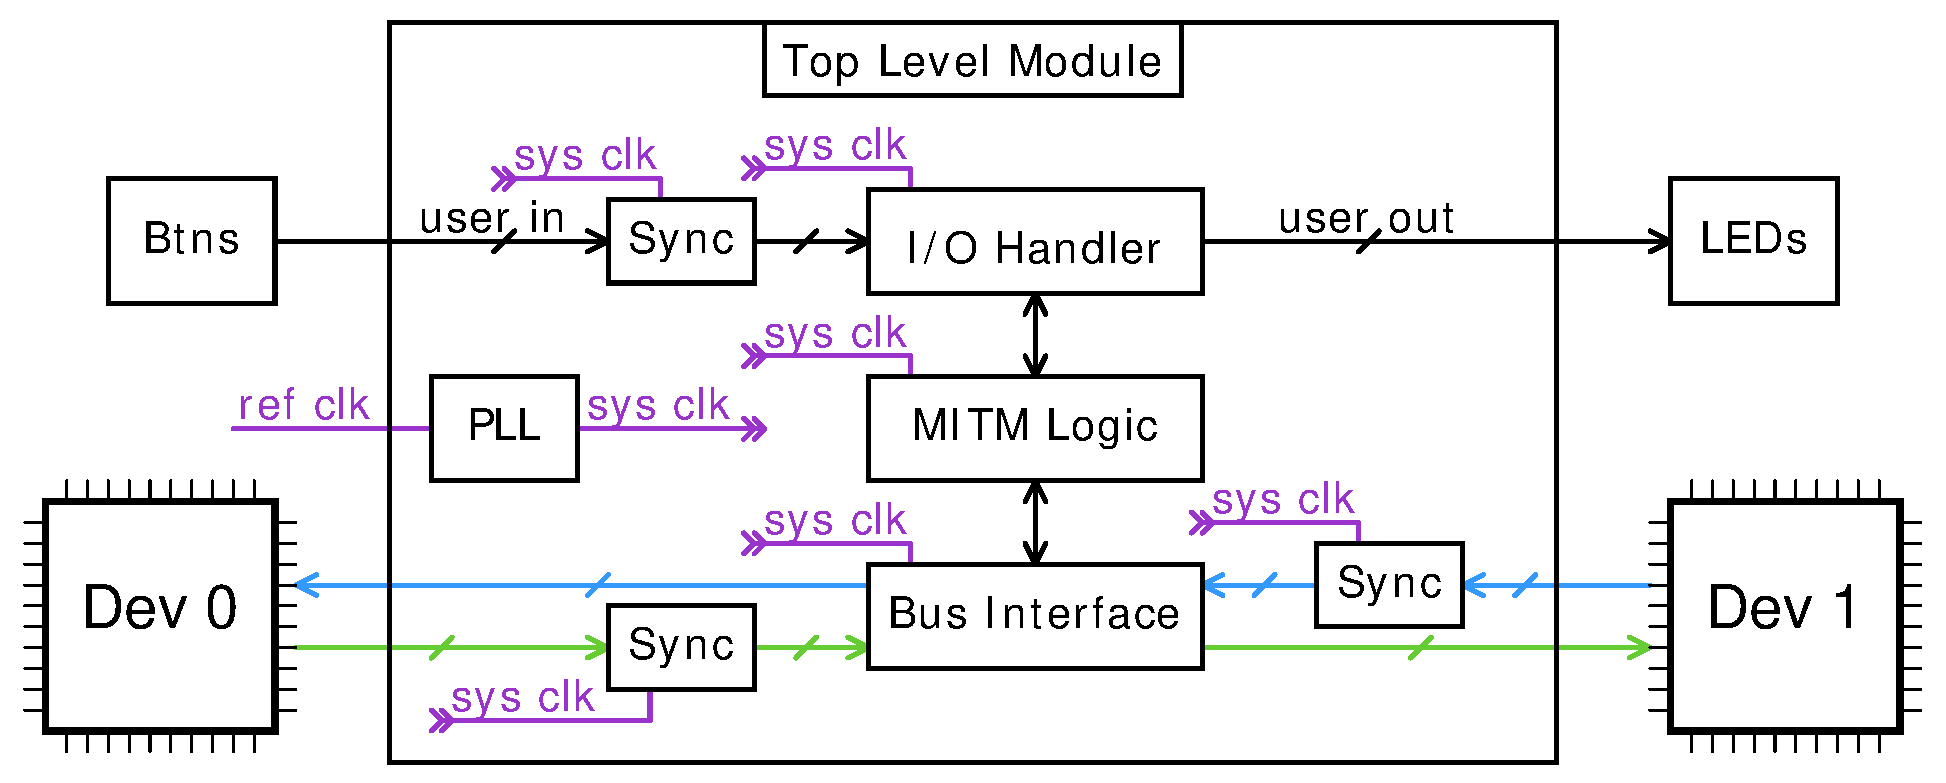
\includegraphics[width=1\textwidth]{images/designs/topLevelModule.pdf}}
    \caption[Schéma hlavného modulu MITM obvodu]{Schéma hlavného modulu MITM obvodu. Komponenty mimo rámu hlavného modulu sú externé a nie sú súčasťou FPGA obvodu. Dev 0 a Dev 1 reprezentujú zariadenia, medzi ktorými chceme realizovať MITM útok.}
    \label{obr:topLevelModule}
\end{figure}

\section{Zbernicové rozhranie pre MITM logiku} \label{sek:busInterface}
Najvýznamnejšou časťou našej implementácie je zbernicové rozhranie, pre MITM logiku, prostredníctvom ktorého možno vykonávať operácie nad komunikáciou. Cieľom rozhrania je zakryť detaily konkrétnej zbernice, ktorej protokol je fyzicky implementovaný na nižšej vrstve. Ako sme spomenuli v časti \ref{sek:masterSlave}, master-slave architektúru nie je možné na tejto úrovni abstrahovať, preto ju ponecháme na vyššiu vrstvu (MITM logika). Schéma, znázorňujúca princíp zapojenia zbernicového rozhrania je na obrázku \ref{obr:busInterface}.

\begin{figure}
    \centerline{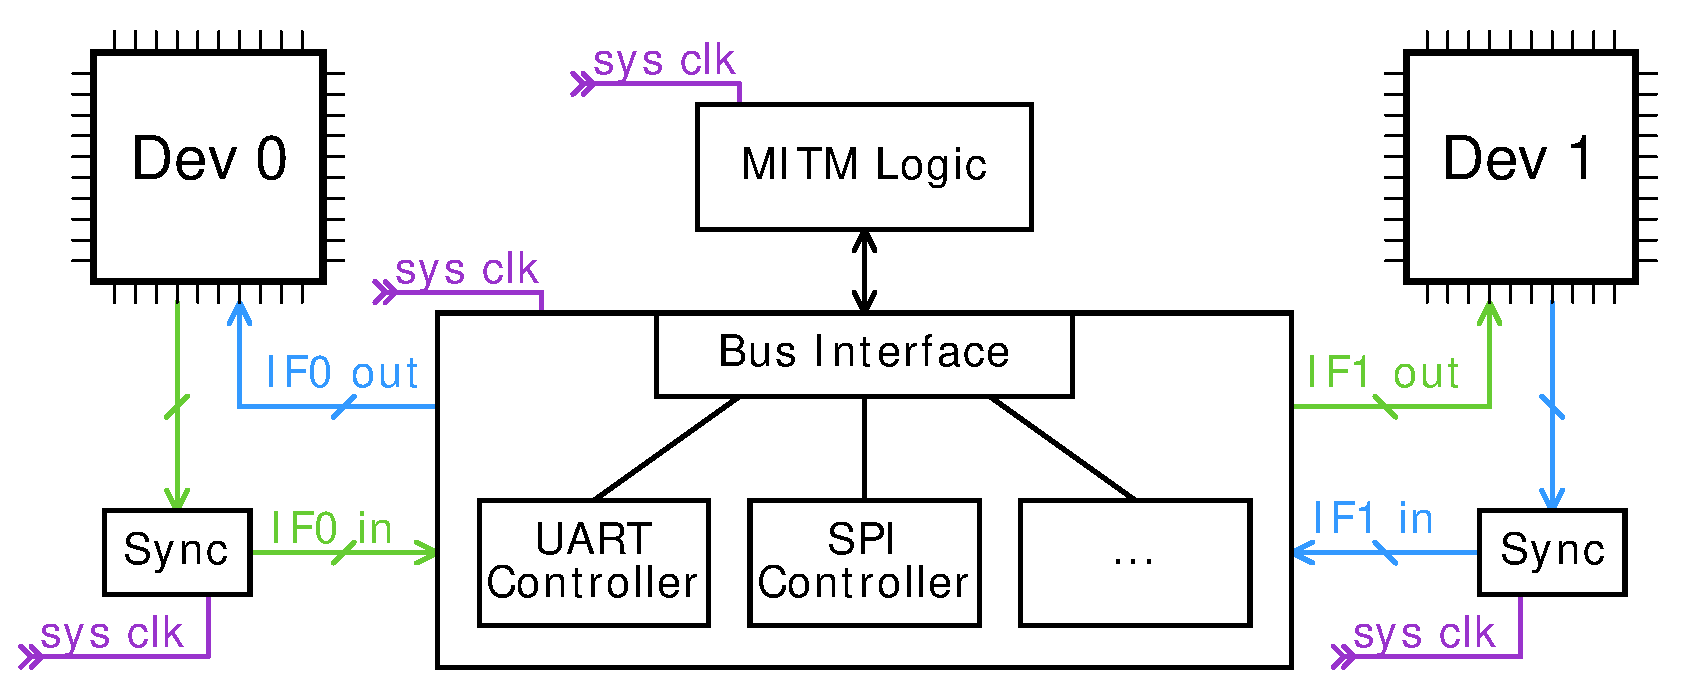
\includegraphics[width=1\textwidth]{images/designs/busInterface.pdf}}
    \caption[Schéma zapojenia zbernicového rozhrania]{Schéma zapojenia zbernicového rozhrania. IF0 a IF1 predstavujú fyzické rozhrania ku skutočným zariadeniam. Vstupné a výstupné linky pre jednotlivé rozhrania sa môžu líšiť v závislosti od konkrétnej zbernice a môžu byť asymetrické (master-slave architektúra). Zariadenia Dev 0 a Dev 1 sú znázorné kvôli prehľadnosti zapojenia a nie sú súčasťou FPGA obvodu.}
    \label{obr:busInterface}
\end{figure}

Cieľom rozhrania je abstrahovať najmä od fyzických vlastností ako napríklad spôsob kódovania logických hodnôt napätím, správna interpretácia prečítaných dát, vysielanie dát, generovanie hodinových signálov v prípade synchrónnej komunikácie a pod. Smerom k vyššej vrstve bude poskytovať rozhranie vstupy a výstupy pre vykonávanie MITM zásahov, prípadne pasívneho odpočúvania. Definícia vstupov a výstupov relevantných pre MITM logiku zbernicového rozhrania v jazyku Verilog je opísaná v algoritme \ref{alg:busInterface}. V tejto časti ho ďalej bližšie vysvetlíme.

\begin{lstlisting}[float,language=Verilog,caption={Definícia vstupov a výstupov zbernicového rozhrania pre MITM logiku. Parameter NUM\_DATA\_BITS nastaví veľkosť bloku prijímaných/vysielaných dát.},label=alg:busInterface]
// riadiace vstupy
input wire fake_if0_select,     // zapne falošný mód na IF1->IF0
input wire fake_if1_select,     // zapne falošný mód na IF0->IF1
input wire fake_if0_send_start, // spustí vysielanie falošných dát
input wire fake_if1_send_start, // spustí vysielanie falošných dát
input wire fake_if0_keep_alive, // zapne keep-alive na IF0
input wire fake_if1_keep_alive, // zapne keep-alive na IF1

// statusové výstupy
output wire if0_recv_new_data,  // signalizuje prijatie nových dát
output wire if1_recv_new_data,  // signalizuje prijatie nových dát
output wire fake_if0_send_ready,// IF0 je pripravené vysielať   
output wire fake_if1_send_ready,// IF1 je pripravené vysielať   
output wire fake_if0_send_done,// signalizuje úspešné odvysielanie
output wire fake_if1_send_done,// signalizuje úspešné odvysielanie

// samotné vysielané/prijímané dáta
input wire [NUM_DATA_BITS-1:0] fake_if0_send_data, // falošné dáta
input wire [NUM_DATA_BITS-1:0] fake_if1_send_data, // falošné dáta
output wire [NUM_DATA_BITS-1:0] real_if0_recv_data,// skutočné dáta
output wire [NUM_DATA_BITS-1:0] real_if1_recv_data,// skutočné dáta
\end{lstlisting}

Základ tvoria vstupy a výstupy pre získanie dát prijatých na obidvoch fyzických rozhraniach zbernice a odvysielanie falošných dát na zvolenom rozhraní, prípadne oboch. Veľkosť (počet bitov) jedného bloku dát je možné nastaviť statickým parametrom. Pri niektorých zberniciach ako UART je táto veľkosť priamo určená parametrom protokolu, a treba ju príslušne nastaviť.

Zbernicové rozhranie ďalej poskytuje rozhranie možnosť prepínania medzi transparentným (forward) režimom a falošným (fake) režimom. Pri transparentnom režime je vysielanie falošných dát ignorované a zbernicové rozhranie fyzicky prepojí vstupy jednej strany na výstupy druhej strany. Tento mechanizmus je realizovaný pomocou multiplexora, ktorý opíšeme v časti \ref{subsek:multiplexor}. Vo falošnom režime rozhranie blokuje skutočnú komunikáciu a na výstupy pripojí falošné linky, po ktorých tečú falošné dáta, ktoré má pod kontrolou MITM logika. V prípade, že chceme komunikáciu iba blokovať, stačí zapnúť falošný režim a riadiaci vstup pre odvysielanie nastavených falošných dát ponecháme na logickej hodnote 0 (falošné dáta sa nikdy neodvysielajú).

Posledný mechanizmus, ktorý naše rozhranie umožňuje je tzv. keep-alive režim. Tento mechanizmus má význam pri zbernicových protokoloch, ktoré na fyzickej vrstve používajú nejaký mechanizmus tzv. relácie (angl. session), v rámci ktorej môže byť odvysielaných niekoľko blokov dát. Príkladom je zbernica SPI, pri ktorej môže master strana ponechať linku SS aktívnu po dlhšiu dobu a v rámci tohoto intervalu môže prebehnúť niekoľko výmen dátových blokov. V prípade, že režim keep-alive je zapnutý ponechá FPGA implementácia konkrétnej zbernice reláciu aktívnu a bude čakať na ďalšie inštrukcie z vyššej vrstvy. Napríklad v prípade SPI zbernice to znamená, že linka SS zostane aktívna aj po odvysielaní falošných dát a SPI implementácia bude čakať na riadiaci vstup pre odvysielanie ďalšieho bloku dát. Mechanizmus keep-alive nie je aplikovateľný na rozhraní, kde simulujeme slave stranu, nakoľko reláciu vždy riadi master.

Na slave strane je naopak potrebné zabezpečiť, aby sa falošné dáta odvysielali v správnom okamihu (komunikáciu riadi master). Pre tento účel využijeme binárny statusový výstup, ktorý indikuje, či je rozhranie na danej strane pripravené vysielať dáta. Implementácia rozhrania môže týmto výstupom signalizovať, že nie je pripravené odvysielať ďalšie dáta, napríklad z dôvodu, že aktuálne práve vysiela predošlé dáta. Implementácia rozhrania na slave strane zároveň bude signalizovať, že nie je pripravená odvysielať dáta aj v prípade, že to momentálne konkrétny master-slave protokol neumožňuje napriek tomu, že slave strana aktuálne nie je činná.

\section{Primitíva}
Pre implementáciu jednotlivých častí obvodu je užitočné postaviť základné primitíva, parametrizovateľné obvody realizujúce jednoduché funkcie. Tento prístup umožní prehľadnejšiu štruktúru kódu a jednoduchšie testovanie a overovanie funkčnosti jednotlivých modulov. V tejto časti stručne opíšeme jednotlivé primitívne obvody, z ktorých budú poskladané zložitejšie moduly.

\subsection{Detektor hrán}
Prvé primitívum, ktoré spomenieme je detektor hrán. Detekcia hrán je potrebná najmä pre rozpoznanie začiatku komunikácie, prípadne konkrétnej fázy v komunikačného protokolu, ktorá vždy začína zmenou signálu (hranou) na niektorej zo vstupných liniek v závislosti od zbernice. Ako mechanizmus detekcie hrán použijeme štandardný prístup. Obvod pre detekciu hrán bude vzorkovať vstup s frekvenciou systémových hodín, pričom si bude pamätať logickú hodnotu signálu pri poslednom prečítaní. Vstupný signál musí byť synchronizovaný so systémovými hodinami. Pokiaľ je pri nasledujúcom čítaní hodnota signálu rôzna od naposledy zapamätanej, detegovali sme hranu, čo signalizujeme na výstup. Obvod umožňuje vybrať parametrom, či chceme chceme detegovať nábehovú alebo dobehovú hranu. Na obrázku \ref{obr:edgeDetectSim} ako príklad uvádzame priebeh signálov počas simulácie detekcie dobehovej hrany.

\begin{figure}
    \centerline{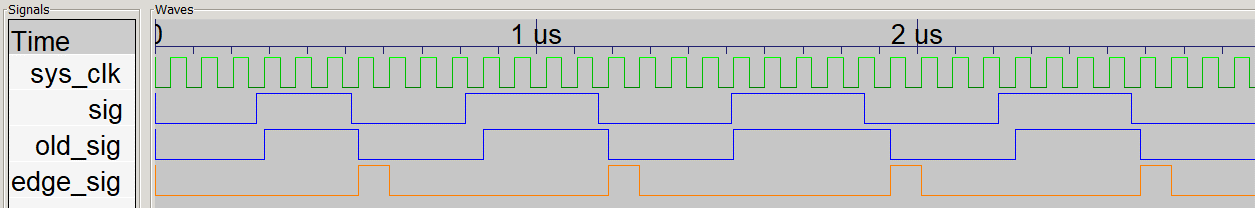
\includegraphics[width=1\textwidth]{images/simulations/edgeDetectSim.png}}
    \caption[Simulácia detekcie dobehovej hrany]{Simulácia detekcie dobehovej hrany. Znázornené signály sú (zhora): systémové hodiny (sys\_clk), aktuálny signál na vstupe (sig), signál zapamätaný pri poslednom čítaní (old\_sig), výstupný signál detekcie (edge\_sig). Pri simulácii vstupy pre jednoduchosť testovania nie sú synchronizované so systémovými hodinami.}
    \label{obr:edgeDetectSim}
\end{figure}

\subsection{Výstupný multiplexor}\label{subsek:multiplexor}
Výstupný multiplexor bude veľmi jednoduchý kombinačný obvod, ktorý multiplexuje medzi dvomi sadami vstupov. Tie predstavujú skutočný signál prijatý na linkách zbernice a falošný signál vygenerovaný zbernicovou implementáciou z dát prichádzajúcich z MITM logiky. Tretím vstupom do multiplexora je selektor, ktorý predstavuje bitovú masku určujúcu, na ktoré linky majú byť nastavené no falošnom režime. Výstupom je multiplexovaná linka v závislostí od nastaveného selektora. Šírka jednotlivých vstupov a výstupu daná počtom liniek zbernice (parameter).

\subsection{Sériový buffer pre čítanie a zápis}
Ďalšími dvoma stavebnými prvkami sú vyrovnávací obvod, ďalej len buffer, pre čítanie, resp. zápis. Cieľom je umožniť čítanie sériových dát na vstupných zbernicových linkách po väčších blokoch a rovnako sériové vysielanie dát na výstupných linkách, ktoré z vyššej vrstvy prichádzajú po blokoch. Užitočným parametrom (pre čítací aj zapisovací buffer) je možnosť nastaviť poradie, v ktorom sa čítajú/zapisujú. Poradie môže byť od najvýznamnejšieho bitu alebo od najmenej významného. Druhým parametrom je veľkosť buffra.

Buffer pre čítanie má ako vstup sériovú linku (synchronizovanú so systémovými hodinami). Ďalej má vstup, ktorý riadi čítanie prostredníctvom jedno-taktových impulzov. Princíp fungovania je nasledovný: Štartovacím riadiacim vstupom sa spustí čítanie a buffer sa nastaví do režimu, kedy čaká na riadiace impulzy pre čítanie. Synchrónne s týmito impulzmi postupne číta logickú hodnotu signálu a ukladá do internej pamäte. Po prečítaní poslednej hodnoty (počet určuje parameter veľkosti buffra) sa čítanie skončí a buffer signalizuje, že prečítané dáta (výstup) sú platné a vyššia vrstva ich môže prevziať.

Buffer pre zápis funguje analogicky. Vstupom je tento krát blok dát, ktorý chceme sériovo odvysielať na výstupnej linke. Rovnako má vstup pre riadenie zápisu prostredníctvom impulzov ako v prípade čítacieho buffra. Princíp fungovania je podobný ako v predchádzajúcom prípade s drobným rozdielom. Cieľom je tento krát podržať logickú hodnotu signálu na výstupnej linke dostatočne dlho (záleží od zbernice), aby ju druhá strana mohla prijať. Prvý bit sa preto na výstup zapíše s polu so spustením zápisu (riadené štartovacím vstupom). Ďalej s každým riadiacim impulzom pre zápis sa výstupná hodnota signálu zmení na nasledovný bit, ktorý chceme odvysielať. Po poslednom zápise buffer podrží hodnotu signálu na výstupe a čaká na posledný zápisový impulz, po ktorom zápis končí. Keďže prvý bit bol zapísaný súčasne so spustením zápisu celý proces bude mať rovnako zápisových impulzov ako je čítacích impulzov v prípade čítacieho buffra. Priebeh signálov počas simulácie činnosti buffrov je znázornený na obrázku \ref{obr:bufferSim}.

\begin{figure}
    \centering
    \subfloat[Buffer pre čítanie. Signály sú (zhora): systémové hodiny (sys\_clk), štartovací signál (start), riadiace impulzy pre čítanie (read\_sig), vstupný sériový signál (in\_line), dáta prečítané v buffri (data\_out), výstupný signál \uv{prečítané dáta sú platné} (done\_sig).]{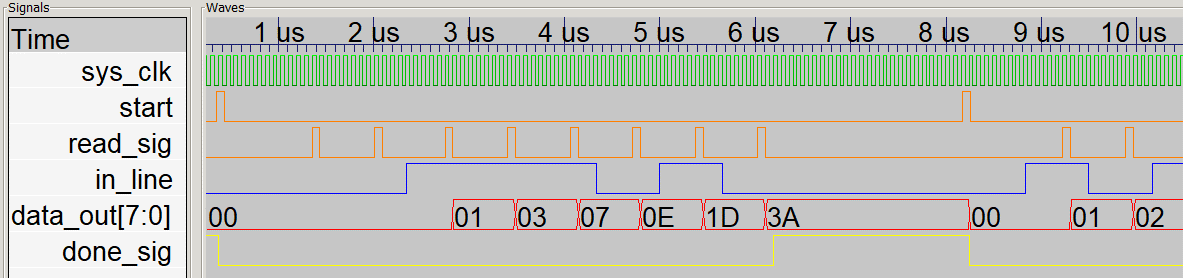
\includegraphics[width=1\textwidth]{images/simulations/readBufferSim.png}}
    \vfill
    \subfloat[Buffer pre zápis. Signály sú (zhora): systémové hodiny (sys\_clk), vstupné dáta pre zápis (data\_in), štartovací signál (start), riadiace impulzy pre zápis (write\_sig), výstupný sériový signál (out\_line), dáta v internom registri, ktoré ešte treba zapísať (write\_buf), výstupný signál \uv{dáta úspešne zapísané}, resp. \uv{buffer pripravený pre zápis} (done\_sig).]{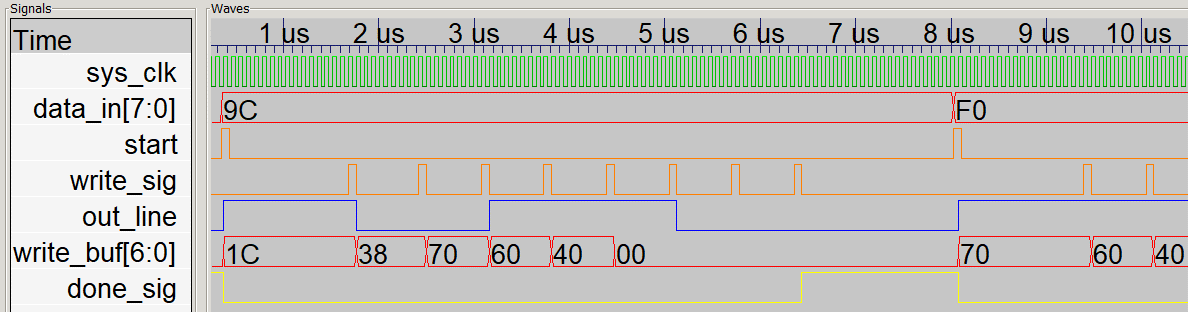
\includegraphics[width=1\textwidth]{images/simulations/writeBufferSim.png}}
    \caption[Simulácia buffrov pre čítanie a zápis]{Simulácia buffrov pre čítanie a zápis. Na vrchnom obrázku je znázornený priebeh signálov pri čítaní, na spodnom priebeh pri zápise/vysielaní. V obidvoch príkladov sú dáta vysielané od najvýznamnejšieho bitu.}
    \label{obr:bufferSim}
\end{figure}

\subsection{Čítač}
Ďalším pomocným obvodom je štandardný čítač. Vstupom je riadiaci signál pre štart a hodnota $n$. Po prijatí štartovacieho signálu čítač začne postupne inkrementovať interný register (inicializovaný na 0), kým nedosiahne hodnotu $n$. Následne sa čítač zastaví a nastaví statusový výstup signalizujúci koniec. Tento mechanizmus je užitočný pre realizáciu oneskorení, ktoré použijeme na dodržanie časových medzier potrebných v závislosti od protokolu zbernice. Napríklad implementácia SPI zbernice môže definovať minimálny časový interval medzi prepnutím SS linky do aktívneho stavu a prvou hranou na hodinách (SCLK).

\subsection{Generátor impulzov}
Posledným primitívom, ktoré využijeme je generátor impulzov. Generátor impulzov je vzásade upravený PVM obvod. Obvod má viacero nastaviteľných parametrov, ktoré definujú vlastnosti vygenerovaného signálu. Hlavné dva parametre sú CYCLE\_COUNT, ktorý určuje počet generovaných impulzov a CYCLE\_LEN, ktorý určuje dĺžku jednej periódy v počte taktov systémových hodín. Vplyv ostatných parametrov na priebeh vygenerovaného signálu je znázornený na obrázku \ref{obr:pulseGen}. Cieľom tohoto obvodu je umožniť jednoduché generovanie riadiacich impulzov s periodickým charakterom. Príkladom sú impulzy pre čítanie a zápis buffrov spomenutých v predošlej časti.

\begin{figure}
    \centerline{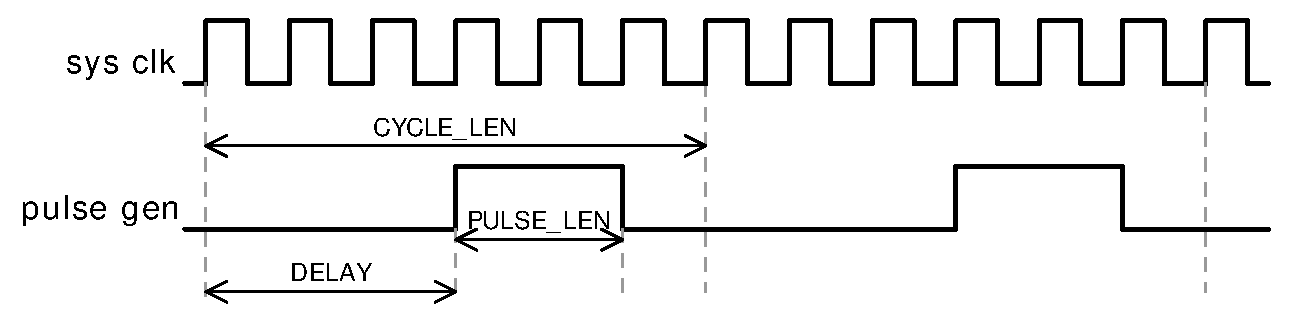
\includegraphics[width=1\textwidth]{images/signals/pulseGen.pdf}}
    \caption[Vizualizácia parametrov generátora impulzov]{Vizualizácia parametrov generátora impulzov. Na vrchu je signál systémových hodín, v spodnej časti je signál vygenerovaný generátorom. Generovaný signál sa periodicky opakuje, pričom počet opakovaní je určený parametrom CYCLE\_COUNT. Následne sa vráti do pasívneho stavu.}
    \label{obr:pulseGen}
\end{figure}

\section{Vstup a výstup}
V tejto časti rozoberieme spôsob spracovania vstupu a výstupu v našej implementácii. Najskôr spomenieme dve techniky -- synchronizáciu a odstraňovanie zákmitov signálu (angl. signal debouncing), ktoré sme použili pri spracovaní vstupov. Obidve tieto funkcionality sú implementované v príslušnom samostatnom module, ktoré popíšeme v častiach \ref{subsek:synchronizer} a \ref{subsek:debouncer}. Takto predspracované vstupy sú následne použité aj v module I/O handler, ktorý spracováva vstup z tlačidiel a generuje výstupné signály pre LED diódy.

\subsection{Synchronizátor} \label{subsek:synchronizer}
V časti \ref{sek:topLevelModule} sme spomenuli potrebu synchronizácie externých vstupov. Táto synchronizácia bude zabezpečená pomocou špeciálneho obvodu -- synchronizátora. Signály z externých vstupov môžu meniť svoj stav nezávisle od internej štruktúry obvodu na FPGA. Preto nie je možné pomocou plánovacieho nástroja (Place and Route) zabezpečiť synchronizáciu týchto zmien so systémovými hodinami ako sme spomenuli v časti \ref{subsek:software}. Pre tento účel je potrebné zabezpečiť synchronizáciu na úrovni logiky obvodu.

Použijeme štandardný prístup synchronizácie jendobitového vstupu. Zreťazíme viacero pamäťových členov, cez ktoré sa bude signál postupne propagovať. Pri porušení časových obmedzení asynchrónnou zmenou signálu na vstupe prvého pamäťového člena môže nastať jedna z troch situácií:
\begin{enumerate}
    \item Napriek porušeniu časovania bude stav pamäte korektne aktualizovaný. Tento prípad nepredstavuje žiadny problém.
    \item Stav pamäťového člena nebude aktualizovaný a ostane v pôvodnom stave. Tento prípad podobne nepredstavuje problém nakoľko v ďalšom takte bude hodnota signálu opäť prečítaná. V najhoršom prípade detegujeme zmenu o jeden takt neskôr.
    \item Pamäťový člen sa dostane do tzv. metastabilného stavu, ktorý má nedefinovanú úroveň napätia. Po konečnom čase, ktorý nie je ohraničený, interný stav konverguje k hodnote logickej 0 alebo 1. Tento prípad je najproblematickejší, nakoľko metastabilita sa môže propagovať do nasledujúcich pamäťových členov v reťazi. Pravdepodobnosť, že bude propagovaná do nasledujúceho člena je pomerne nízka, v závislosti od hardvéru až zanedbateľná. Túto pravdepodobnosť možno ďalej exponenciálne znížiť pridaním ďalších pamäťových členov v reťazi. Štandardne sa na synchronizáciu používa reťaz dĺžky 2--3 členov \cite{metastability}.
\end{enumerate}
Princíp metastability a synchronizácie pomocou reťaze pamäťových členov je znázornený na obrázku \ref{obr:synchronizer}.

\begin{figure}
    \centering
    \subfloat[Synchronizačná reťaz pamäťových členov.]{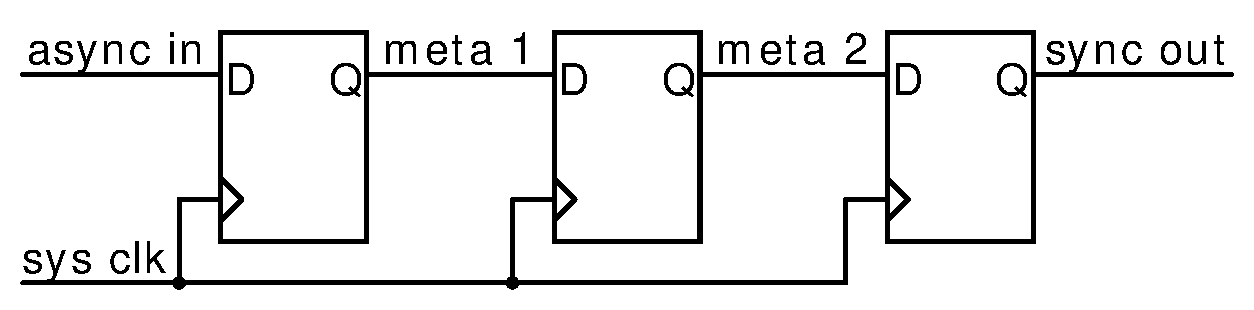
\includegraphics[width=1\textwidth]{images/designs/synchronizer.pdf}}
    \vfill
    \subfloat[Priebeh signálov počas synchronizácie. Pri prvej asynchrónnej zmene vstupu (T1) sa prvý člen (meta 1) dostal do metastabilného stavu. \uv{Zotavil} sa dostatočne rýchlo preto sa metastabilita nepropagovala ďalej v reťazi. V druhom prípade (T4) sa metastabilita propagovala o jeden člen ďalej (T4--T6). Situácia v druhom prípade je veľmi zriedkavá.]{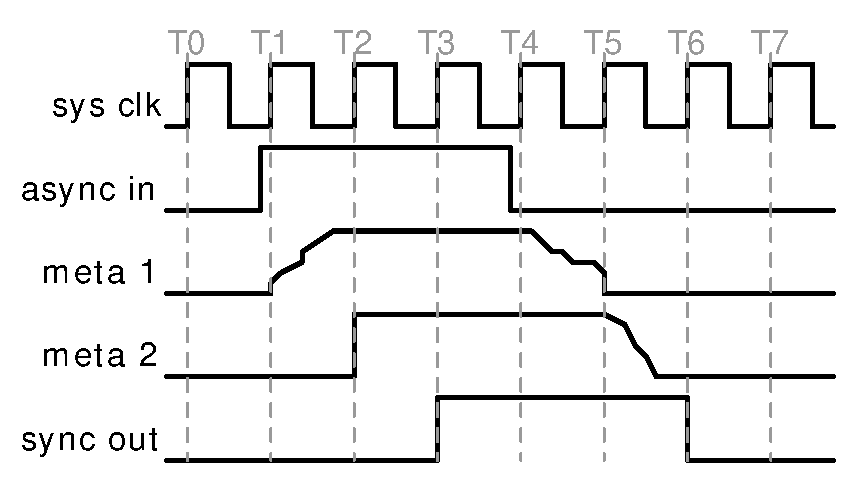
\includegraphics[width=0.9\textwidth]{images/signals/metaSignals.pdf}}
    \caption[Synchronizácia a metastablilita]{Synchronizácia a metastablilita. Na hornom obrázku je znázornená schéma synchronizačného obvodu pre jednobitový asynchrónny vstup. Na spodnom obrázku možno vidieť príklad priebehu jednotlivých signálov v prípade metastability jednotlivých pamäťových členov.}
    \label{obr:synchronizer}
\end{figure}

Obvod synchronizátor potom bude pozostávať z reťazi dvoch pamäťových členov pre každý zo vstupných signálov, ktorých počet je možné nastaviť parametrom. Zdôrazňujeme, že tento prístup nezabezpečuje synchronizovanú zmenu naprieč viacerými jednobitovými vstupmi. V našom prípade to nie je problém, nakoľko všetky externé vstupy, sú jednobitové a navzájom od seba nezávislé pre ostatnú logiku obvodu. Pokiaľ by sme mali vstup pozostávajúci z viacerých závislých bitov, napr. 32-bitová reprezentácia čísla, potrebovali by sme zabezpečiť, že zmena bude detegovaná súčasne na celom vstupnom slove. Príkladom môže byť použitie tzv. guard vstupu -- jednobitový vstup (ten je potrebné synchronizovať), ktorý signalizuje, že ostatné vstupy sú stabilné a je bezpečné ich prečítať. Sémantiku guard signálu je potrebné zabezpečiť logikou synchronizátora, prípadne obvodu, z ktorého prijímame vstup.

\subsection{Odstránenie zákmitov signálu} \label{subsek:debouncer}
Ďalším problémom je spracovanie vstupov z externých tlačidiel. Tlačidlo pri stlačení/uvoľnení zvyčajne generuje \uv{skákavý} signál, meniaci logický stav medzi 0 a 1. Ten môže spôsobiť, že jedno stlačenie/uvoľnenie detegujeme niekoľkonásobne viackrát. Odstránenie takýchto zákmitov signálu je na FPGA pomerne jednoduché. Aj krátke stlačenie tlačidla predstavuje pomerne veľký časový interval z pohľadu rýchlosti FPGA, rádovo minimálne desiatky milisekúnd. Na vstupnom signále budeme preto počítať čas od poslednej hrany (v počte taktov systémových hodín). Pokiaľ je tento čas dostatočne veľký, signál na vstupe je stabilný, teda jeho hodnotu považujeme za platnú a môžeme ju spracovať. Pokiaľ je takto stabilný signál v aktívnom stave (logická 0 alebo 1 v závislosti od nastavenia parametra), pošleme na výstup signál, že sme detegovali stlačenie tlačidla. Simulácia signálov spracovania slačenia tlačidla je na obrázku \ref{obr:debouncerSim}. Vstup z tlačidla je potrebné pred odstránením zákmitov, rovnako ako ostatné vstupy, synchronizovať.

\begin{figure}
    \centerline{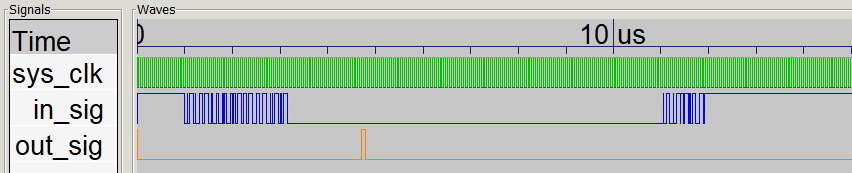
\includegraphics[width=1\textwidth]{images/simulations/debouncerSim.png}}
    \caption[Simulácia spracovania vstupu z tlačidla]{Simulácia spracovania vstupu z tlačidla. Signály sú (zhora): systémové hodiny (sys\_clk), vstupný signál z tlačidla (in\_sig), výstupný signál stlačenia (out\_sig). Kvôli kratšej simulácii trvá simulované stlačenie len niekoľko mikrosekúnd, v skutočnosti je rádovo dlhšie (minimálne desiatky milisekúnd).}
    \label{obr:debouncerSim}
\end{figure}

\subsection{I/O handler}
Posledný modul v rámci vstupu a výstupu je I/O handler. Úlohou tohoto obvodu je spracovať vstupy od tlačidiel (synchronizované a odstránené o zákmity) a rovnako generovať výstupné signály pripojené k LED diódam. Na vstupe sme implementovali podporu pre dve tlačidlá. Prvým je globálny reset, ktorý sa po prijatí a detegovaní stlačenia v I/O handler propaguje do všetkých ostatných obvodov, pri ktorých je reset zmysluplný. Jednoduché obvody ako napríklad synchronizátor a detektor hrán nepotrebujú byť inicializované v dobre definovanom stave a preto u nich nie je reset vstup potrebný.

Druhým tlačidlom je mód select, ktorým je možné poslať vstup pre MITM logiku. Tento vstup je myslený na umožnenie dynamického prepínania medzi rôznymi režimami MITM logiky. Aktuálne nastavený režim si I/O handler udržuje v internom registri, ktorý je pripojený na vstup MITM logiky. V implementácii MITM logiky je prípadne možné využiť tento vstup aj na iné účely podľa potreby. Hodnota aktuálne nastaveného režimu je zároveň posielaná na výstupné LED diódy, ktoré signalizujú túto hodnotu používateľovi.

Posledná funkcia I/O handler modulu je signalizácia aktuálne prebiehajúcej komunikácie prostredníctvom LED diódy. V závislosti od zbernice sa logika detekcie signálu môže líšiť, preto je táto logika ponechaná na implementáciu zbernice a výstup detekcie je pripojený na vstup pre I/O handler, ktorý ho ďalej spracuje a výsledný signál pošle na výstupnú LED. Schéma pripojenia vstupov a výstupov k modulu I/O handler je na obrázku \ref{obr:ioHandler}.

\begin{figure}
    \centerline{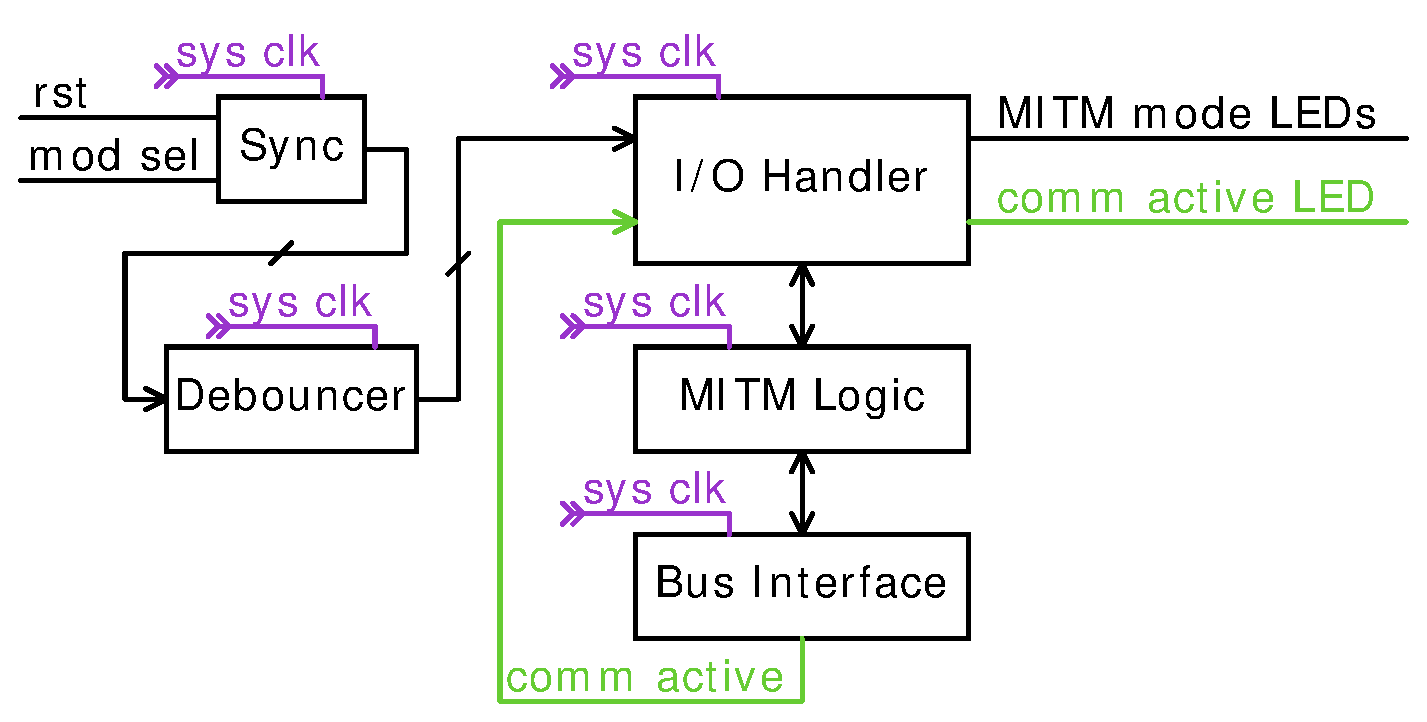
\includegraphics[width=1\textwidth]{images/designs/ioHandler.pdf}}
    \caption[Schéma zapojenia obvodu I/O handler]{Schéma zapojenia obvodu I/O handler.}
    \label{obr:ioHandler}
\end{figure}

\section{Implementácia vybraných zberníc}
V tejto časti opíšeme spôsob implementácie dvoch zberníc, konkrétne UART a SPI. Rozhodli sme sa pre tieto dve zbernice, nakoľko sa líšia v pomerne veľkom množstve vlastností, ktoré sme opísali v kapitole \ref{kap:zbernice}.

\subsection{UART implementácia}
Implementácia UART zbernice bude pomerne priamočiara, nakoľko UART je po hardvérovej stránke pomerne jednoduchý a zároveň komunikácia je symetrická pre obidve strany, čo umožní znovupoužitie kódu pre implementáciu jednej strany. Implementáciu rozdelíme na dva moduly.

Prvým je UART driver, ktorý implementuje štandardný UART protokol pre jednu (ľubovoľnú) stranu. Základnými vstupmi a výstupmi budú linky RX/TX a dáta, ktoré chceme vyslať (TX) a dáta, ktoré sme prijali (RX). Ďalej budeme mať riadiaci vstup pre spustenie vysielania na TX linke a dva statusové výstupy -- prijatie nových dát na RX linke a TX linka pripravená vysielať. Implementácia je potom priamočiara. Čítanie a zápis prebieha nezávisle (UART zbernica je asynchrónna). Na RX linke detegujeme dobehovú hranu (START bit), čo spustí čítanie. Následne spustíme čítací buffer a ako riadiaci vstup pre čítacie impulzy pripojíme výstup z generátora impulzov. Parametre generátora nastavíme tak, aby generoval jednotaktové impulzy približne v strede prijímaného bitu, čo staticky vypočítame pomocou symbolovej rýchlosti tiež nastavenej parametrom. Vysielanie na TX linke je implementované analogicky, pričom použijeme buffer pre zápis a ako štartovací signál použijeme riadiaci vstup pre spustenie vysielania. Schéma UART driver obvodu je na obrázku \ref{obr:uartDriver}.

\begin{figure}
    \centerline{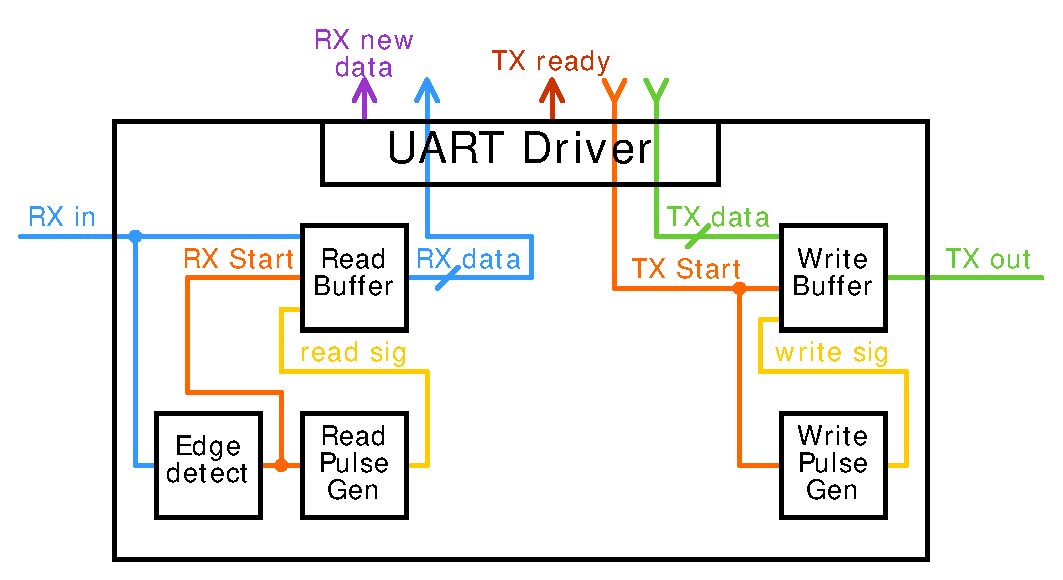
\includegraphics[width=1\textwidth]{images/designs/uartDriver.pdf}}
    \caption[Schéma implementácie UART driver modulu]{Schéma implementácie UART driver modulu.}
    \label{obr:uartDriver}
\end{figure}

Druhým modulom implementácie UART zbernice je UART controller. Jeho úlohou je prepojiť dve inštancie modulu UART driver na príslušných stranách rozhrania zabezpečiť funkcionalitu abstraktného zbernicového rozhrania opísaného v časti \ref{sek:busInterface}. Funkcionalitu prepínaním medzi transparentným a falošným režimom implementujeme pomocou výstupného multiplexora. V transparentnom režime multiplexor pripojí na výstup priamo vstup z jednotlivých RX liniek do kríža (podobne ako je znázornené na obrázku \ref{obr:uartWiring} v kapitole \ref{kap:zbernice}), čo znamená, že komunikácia úplne obíde výstup z UART implementácie nášho obvodu. Čítanie dát na RX linkách bude stále funkčné a bude tak možno komunikáciu pasívne odpočúvať. Vo falošnom prežime multiplexor pripojí na výstup TX výstupy z našej UART implementácie, čo umožní posielanie falošných dát. Mechanizmus keep-alive na zbernici UART nie je aplikovateľný na koľko UART nedefinuje žiadny mechanizmus relácie. Ostatná funkcionalita je pri UART zbernici priamočiara. Schéma zapojenia UART controller obvodu je na obrázku \ref{obr:uartController}.

\begin{figure}
    \centerline{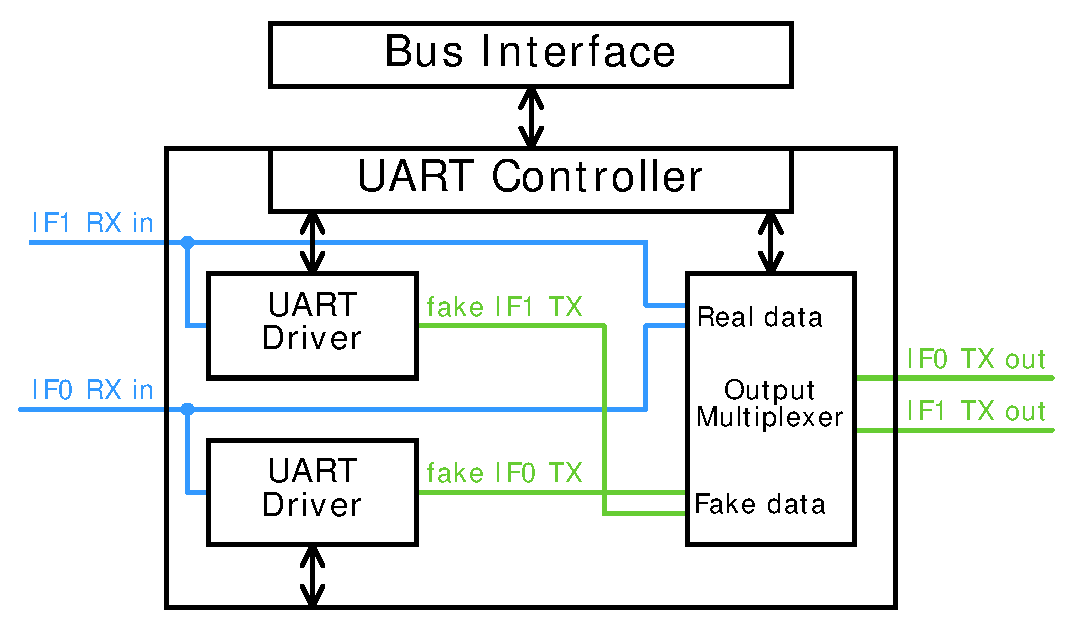
\includegraphics[width=1\textwidth]{images/designs/uartController.pdf}}
    \caption[Schéma obvodu UART controller]{Schéma obvodu UART controller.}
    \label{obr:uartController}
\end{figure}

\subsection{SPI implementácia}
SPI zbernica je na hardvérovej úrovni značne komplikovanejšia v porovnaní s UART zbernicou. Najväčšie komplikácie spôsobuje asymetrickosť master-slave architektúry a jej dôsledky, ktoré sme spomenuli v časti \ref{sek:masterSlave}. Napriek sa nám SPI zbernicu pre MITM útoky podarilo implementovať s tým, že niektoré aspekty tejto architektúry sa presúvajú na vyššiu vrstvu a musí s nimi MITM logika počítať. Podobne ako pri implementácii UART zbernice máme dva základné moduly.

SPI driver je tento krát rozdelený na dva samostatné moduly, jeden implementujúci rozhranie pre slave stranu (sme pripojený mastrovi) a jeden pre master stranu (pripojený k slave skutočnému zariadeniu). Implementácia týchto modulov je po technickej stránke pomerne komplikovaná preto ju nebudeme detailne opisovať a spomenieme len dve zaujímavé myšlienky. Pre podrobnosti implementácie čitateľa odkazujeme na elektronickú prílohu priloženú k práci.

Na slave je potrebné zabezpečiť, aby sme dáta posielali len vo vyhradených časových intervaloch, čo pri SPI zbernici znamená len v momente, keď je SS v aktívnom stave a master začne vysielať hodinový signál. To znamená, že naše okno, kedy musíme začať vysielať je od momentu keď master zapne SS, kým nenastane prvá (v prípade módu 0) nábehová hrana na SCLK linke ako je znázornené na obrázku \ref{obr:spiSlaveWindow}. Túto funkcionalitu zabezpečíme tak, statusový výstup \uv{MISO je pripravené vysielať} budeme signalizovať len počas tohoto intervalu. Mimo okna bude tento výstup vypnutý (logická 0) napriek tomu, že SPI slave driver je aktuálne pasívny -- čaká na možnosť vysielať.

\begin{figure}
    \centerline{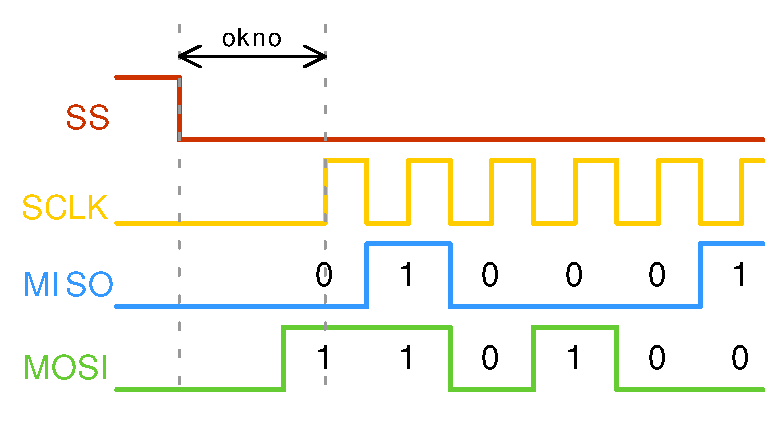
\includegraphics[width=1\textwidth]{images/signals/spiSlaveWindow.pdf}}
    \caption[Okno pre spustenie vysielania SPI slave dát]{Okno pre spustenie vysielania SPI slave dát na MISO linke.}
    \label{obr:spiSlaveWindow}
\end{figure}

Na master strane máme iný zaujímavý problém. V prípade, že odvysielame blok dát, je potrebné rozlíšiť medzi dvoma prípadmi. V prvom chce master ukončiť komunikáciu, čo znamená, že nastaví SS linku do pasívneho stavu. V druhom prípade má komunikácia pokračovať bude odvysielaný ďalší blok dát, pričom medzi blokmi dát môže byť rôzne dlhá prestávka, počas ktorej je SS signál aktívny. Pre rozlíšenie medzi týmito dvomi prípadmi práve využijeme mechanizmus keep-alive, ktorého sémantiku sme opísali v časti \ref{sek:busInterface}. V prípade, že keep-alive vstup je vypnutý (logická 0) ide o prvý prípad a komunikáciu ukončíme nastavením SS linky do pasívneho stavu. Pokiaľ je  keep-alive zapnutí (logická 1) ponecháme SS aktívny a budeme čakať na riadiaci vstup pre odvysielanie ďalšieho bloku dát.

Posledným komponentom v našej SPI implementácii je analogicky ako v UART prípade SPI controller. Jeho úloha je podobná, zabezpečiť funkcionalitu zbernicového rozhrania na vyššej vrstve prepojením potrebných vstupv a výstupov. Podobne ako pri UART implementácii, prepínanie medzi falošným a transparantným režimom zabezpečíme pomocou výstupného multiplexora, ktorý bude mať v tomto prípade viacej liniek (pre každú linku SPI zbernice). Schéma interného zapojenia SPI controller obvodu je na obrázku \ref{obr:spiController}. Nakoľko pri SPI zbernici je jeden smer komunikácie závislý od druhého nie je možné nezávisle na oboch smeroch komunikácie prepínať medzi falošným a transparentným režimom a je potrebné, aby boli súčasne v vždy rovnakom stave.

\begin{figure}
    \centerline{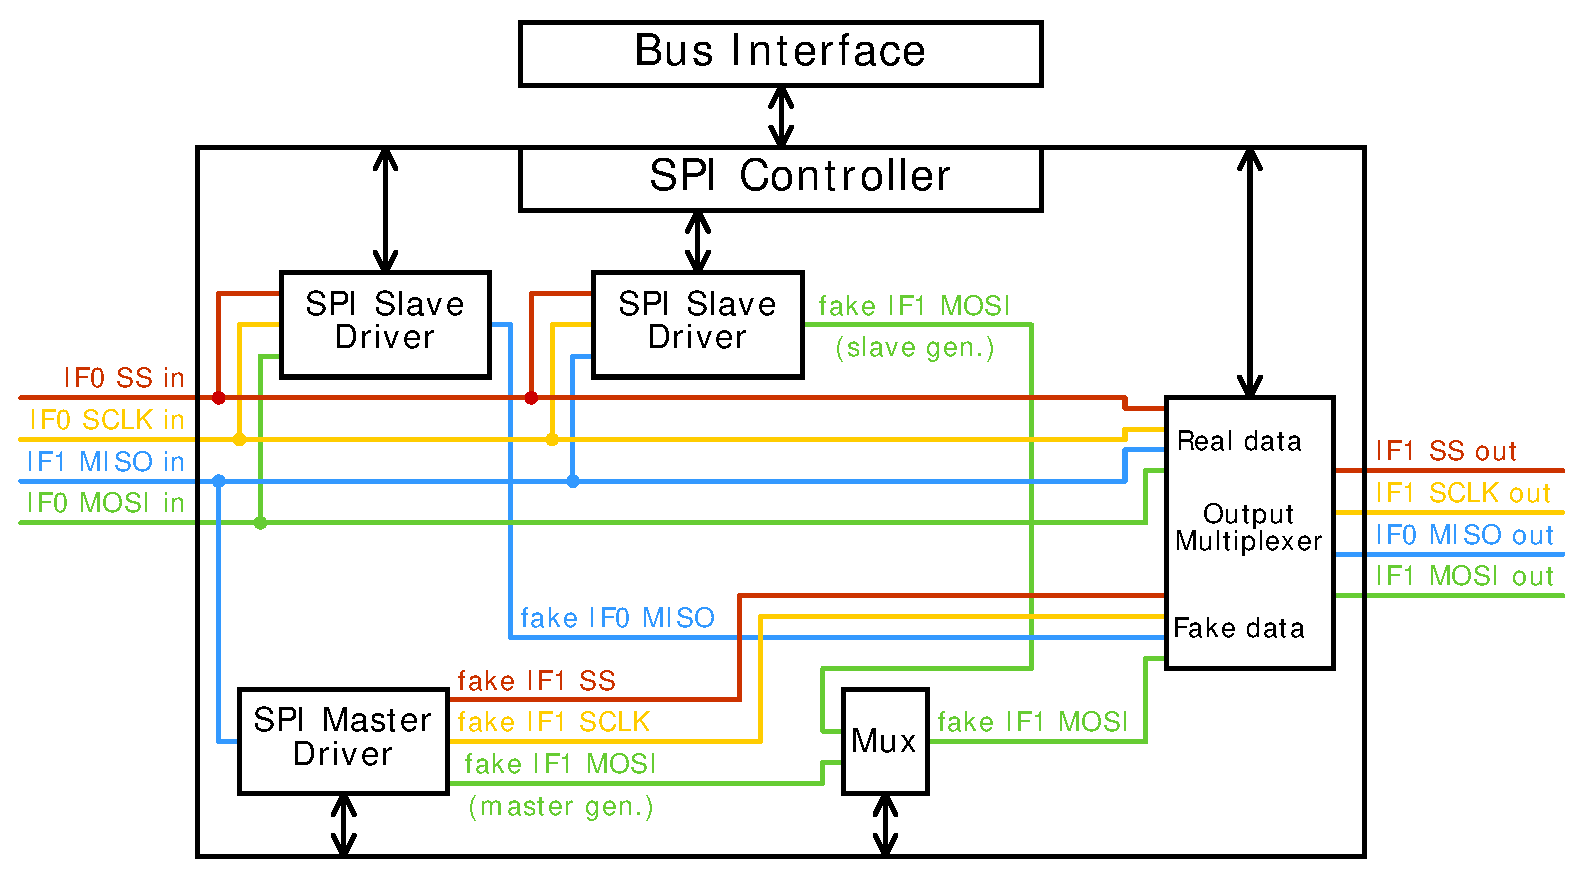
\includegraphics[width=1\textwidth]{images/designs/spiController.pdf}}
    \caption[Schéma obvodu SPI controller]{Schéma obvodu SPI controller.}
    \label{obr:spiController}
\end{figure}

\section{Konfigurácia MITM obvodu}
V tejto časti opíšeme spôsob konfigurácie a vytvorenie finálneho zabalenej konfigurácie, ktorú možno priamo nahrať na zvolenú FPGA dosku. Ako prvé je vhodné nakonfigurovať parametre MITM obvodu v dedikovanom súbore \texttt{config.vh}, ktorý je pripojený v zdrojovom kóde k relevantným modulom. Zoznam konfigurovateľných parametrov je v tabuľke \ref{tab:config}. Niektoré parametre sú špecifické pre konkrétnu zbernicu, preto sú aplikovateľné len v prípade, že je táto zbernica nastavená.

\begin{table}
    \caption[Konfigurovateľné parametre FPGA obvodu]{Konfigurovateľné parametre FPGA obvodu.}
    \label{tab:config}
    \begin{center}
    \begin{tabular}{V{4}c|cV{4}}
        \hlineB{4}
        Parameter & Popis \\
        \hlineB{4}
        \multirow{2}{*}{SYS\_FREQ} & frekvencia systémových hodín v MHz \\
        & (podporovaný rozsah: 16 -- 275 MHz \textsuperscript{(1)}) \\
        \hline
        \multirow{2}{*}{DEBOUNCE\_LEN\_US} & čas v {\textmu}s, kým je stabilný signál tlačidla detegovaný \\
        & (použité pri odstraňovaní zákmitov signálu) \\
        \hline
        NUM\_MITM\_MODES & počet režimov pre MITM logiku (maximálne 4) \\
        \hline
        NUM\_DATA\_BITS & veľkosť bloku dát prenášaných na zbernici \\
        \hline
        UART\_BAUD\_RATE & symbolová rýchlosť pre UART zbernicu \\
        \hline
        SPI\_FREQ\_HZ & frekvenica hodín na SPI zbernici v Hz \\
        \hline
        \multirow{2}{*}{SPI\_SS\_ACTIVE\_LOW} & nastaví polaritu SS linky SPI zbernice \\
        & nenulová hodnota znamená active-low \\
        \hline
        \multirow{2}{*}{SPI\_LSB\_FIRST} & poradie bitov pri prenášaní SPI dát \\
        & nenulová hodnota znamená najnižší bit prvý \\
        \hline
        \hlineB{4}
    \end{tabular}\\
    \textsuperscript{(1)} Nie všetky hodnoty z rozsahu je možné PLL obvodom dosiahnuť. V prípade, že nastavenú frekvenciu nie je možné dosiahnuť, použije sa najbližšia možná.
    \end{center}
\end{table}

Po konfigurácii parametrov je potrebné implementovať MITM logiku podľa potreby použitia obvodu. V kapitole \ref{kap:priklady} predstavíme dve ukážky MITM útokov/zásahov do komunikácie pomocou nášho obvodu, kde uvedieme aj príklad vzorovej implementácie MITM logiky.

Ďalej sa medzi zdrojovými súbormi nachádzajú definície mapovania medzi logickými vstupmi/výstupmi hlavného modulu FPGA obvodu (na úrovni jazyka Verilog) a fyzickými I/O portami FPGA čipu. Tieto definície sú uložené vo formáte PCF a sú logicky rozdelené podľa jednotlivých dosiek (tie majú niektoré I/O porty rôzne) a podľa zbernice (rôzne zbernice majú rôzny počet vstupov/výstupov). Tieto možno upraviť podľa potreby, v prípade, že vyhovujú predvolené nastavenia nie je potrebné ich upravovať. Následne je potrebné dodržať definované I/O porty pri fyzickom zapojení FPGA obvodu. Ukážku fyzického zapojenia demonštrujeme na príkladoch v kapitole \ref{kap:priklady}. 

Za predpokladu, že je MITM logika správne implementovaná a obvod nakonfigurovaný, je možné spustiť skript pre zostavenie (angl. build) výslednej zabalenej konfigurácie pre FPGA, pomocou nástroja GNU make. Skript využíva softvérové nástroje popísané v časti \ref{subsek:software}. Pri spustení skriptu možno zvoliť kombináciu zbernice a jednej z podporovaných dosiek (icestick alebo HX8K). prípadne možno spustiť predvolený cieľ, ktorý zostaví všetky možné konfigurácie. Podrobnejší návod na spšťanie skriptu sa nachádza v súbore \texttt{README.md} v elektronickej prílohe.